\section{Introduction}

This document describes the Tagion core network.\\
The tagion core network includes the byzantine consensus algorithm, the consensus database and description of node validators and the basic node selections. 

\subsection{Network Architecture}
The Tagion network architecture consist of a collections of computer nodes which are able to send messages between each other (A \bfit{computer node} is named \bfit{node} in this document). Each node can send a message to any other node in the network.\\
The nodes in the network has different roles and the nodes will change roles over the lifetime depended controlled by the Tagion consensus rule.\\ 

The node roles are:
\begin{itemize}
	\item[\bfit{Active Node}] The node in this role category takes care of the validations.
	\item[\bfit{Standby Node}] Those nodes are waiting to be selected  as validators.
	\item[\bfit{Swap Node}] Those nodes has been selected to be swapped with an \bfit{Active Node} and become a validator.  
	\item[\bfit{Prospect Node}] Nodes in this category are waiting to become and 'real' node in the network 
	\label{tab:node_roles}
\end{itemize}

All the nodes communicates via protocol call libp2p \cite{libp2p}. The role of the node actors are selected randomly (\bfit{UDR} \cref{sec:SMT}) according to the node consensus selection rules \cref{sec:mutation}.

\begin{figure}[H]
	\centering
	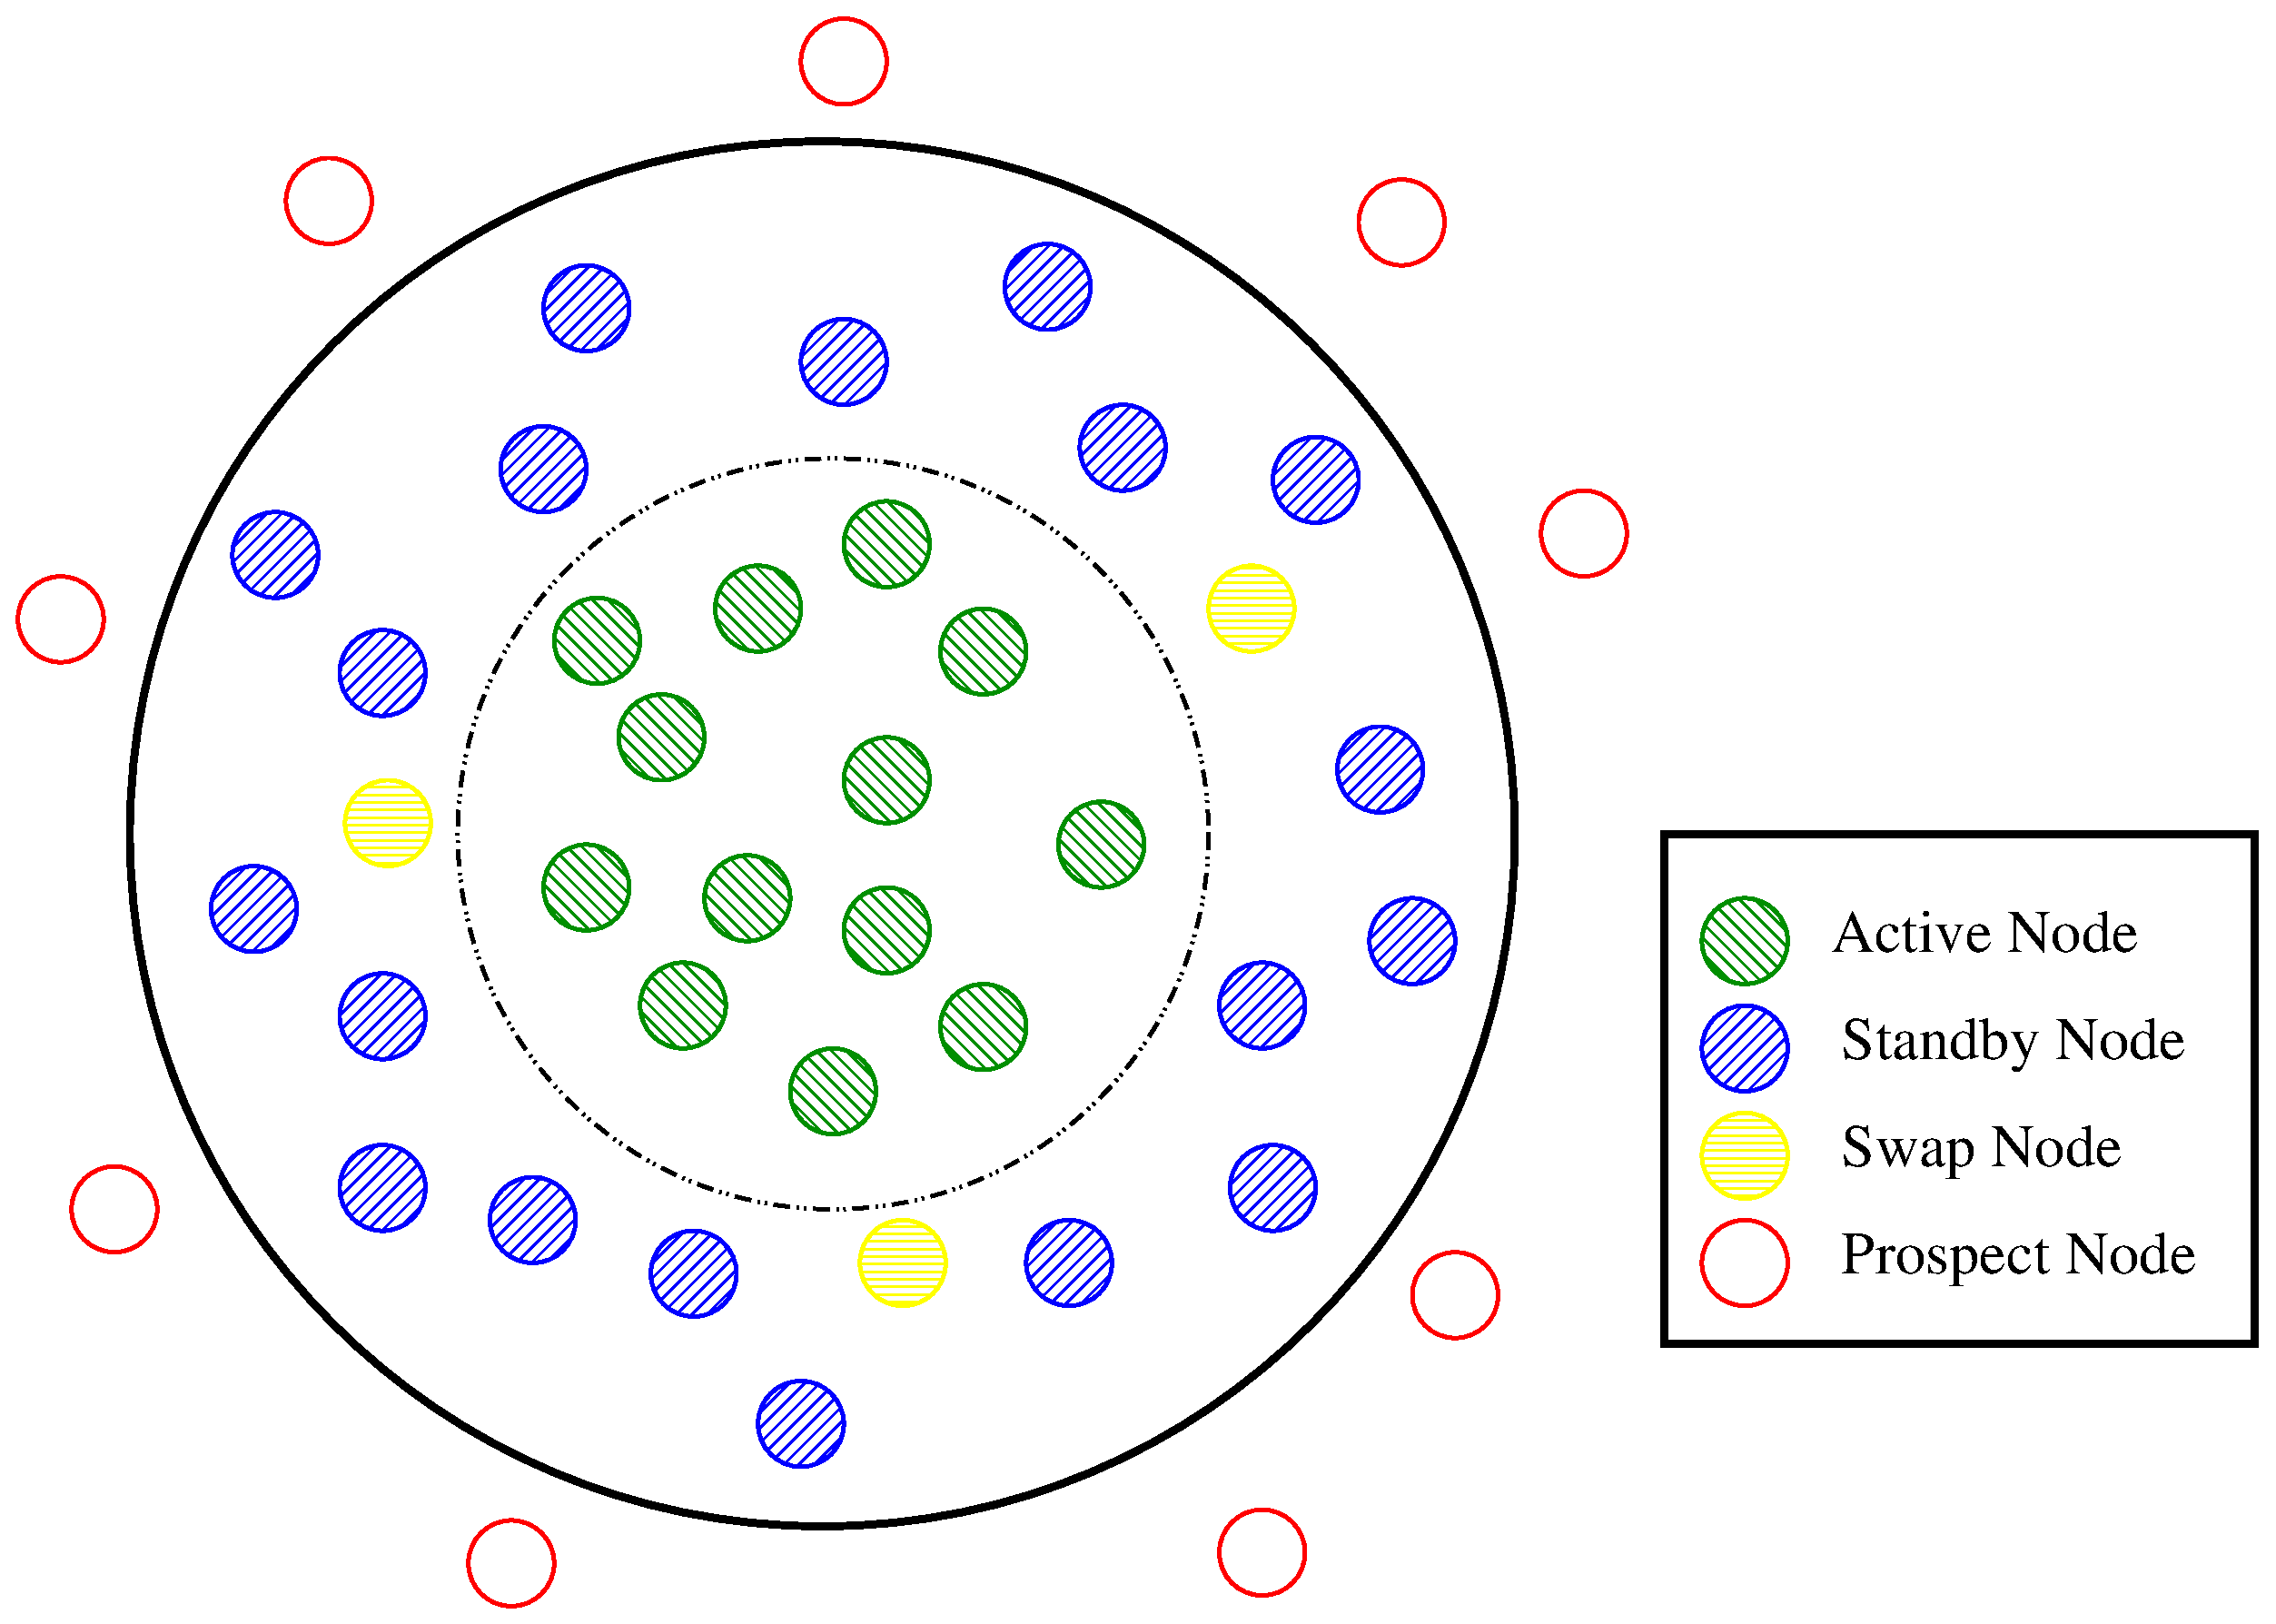
\includegraphics[width=0.8\textwidth]{fig/network_architecture.eps}
	% dart_bw.eps: 17766x12625 px, 300dpi, 150.42x106.89 cm, bb=0 0 4264 3030
	\caption{The Network Architecture}

	\label{fig:network_architecture}
\end{figure}

The \bfit{Active Node}'s validates the transaction and used the Hashgraph algorithm \cref{sec:hashgraph_cm} to reach consensus. The Hashgraph algorithm is capable of producing a consensus order list of transaction (Defined as \bfit{transaction list}). This means that all the \bfit{Active Node}'s will produces the same order of transactions.\\
The transaction list is processed in that order the procedure for execution can be found in \cref{sec:network}.
 
\subsection{Node Architecture}
The node core program is implemented in the programming language D with some C and Go libraries for crypto, network and virtual engine functions. It is structured, as shown in the figure below. 

\begin{table}[H]
	{%
		\newcommand{\mc}[2]{\multicolumn{#1}{#2}}
		\begin{center}
			\begin{tabular}{|c|c|}
				\hline
				\mc{2}{|c|}{HiRPC (HiBON) Dataformat for communication}\\
				\hline
				\mc{2}{|c|}{NODE}\\
				\hline
				User API - TLS 1.2 & P2P Network\\
				\hline
				\mc{2}{|c|}{Tagion Virtual Machine}\\
				\hline
				\mc{2}{|c|}{Consensus mechanism : Hashgraph}\\
				\hline
				\mc{2}{|c|}{Storage : Distributed Database DART }\\
				\hline
				\mc{2}{|c|}{Blockchain : Epoch Records} \\
				\hline
			\end{tabular}
		\end{center}
	}%
	\caption{Tagion Node stack}
	\label{tab:node_stack}
\end{table}


A Tagion Node is divided into units as shown in \cref{fig:node_service} and each unit handles a service function in the following manner:

A smart-contract is sent to the Transaction-service-unit which are fetching the inputs date form the distributed Data-base DART unit (see \cref{sec:DART}) and verifying their signatures of the inputs. The DART-unit connects to other DARTs via the P2P-unit. The transaction-unit forwards the smart-contract to the Coordinator-unit and this unit that is gossiped to the network via the P2P-unit.\\
When the Coordinator receives an event with a smart-contract, the smart-contract contract is verified and executed via the \abbrev{TVM}{Tagion Virtual Machine} unit, and the results of the outputs are verified.\\
The Coordinator adds it to an event in the Hashgraph and gossips the informations via the P2P-unit to other nodes in the network.    
When the Coordinator finds an epoch, it make a list of ordered transactions and forwards this list to the Transcript-service-unit. The transcript-unit executes the smart-contracts in order and produces list called an Recorder. A Recorder is contains list of all the inputs to be erased and all the outputs to be added. The Coordinator send Recorder to the DART-uint which executes this list. The DART-unit forwards the Recorder to the Recorder-unit and the Recorder adds this to a block-chain.\\
In the case that the Coordinator resolves that super majority of the active-nodes dose not agree the Coordinator send an undo-instruction to the Recorder-unit.\\
If the Recorder-unit receives an undo-instruction the recorder will send the Recorder-list in reverse order to the DART-unit and the DART-unit will perform this action and put the DART in the previous state before the last Epoch.
The Logger-unit and the Monitor-unit used for debugging and monitoring the network.

\begin{figure}[H]
	\centering
	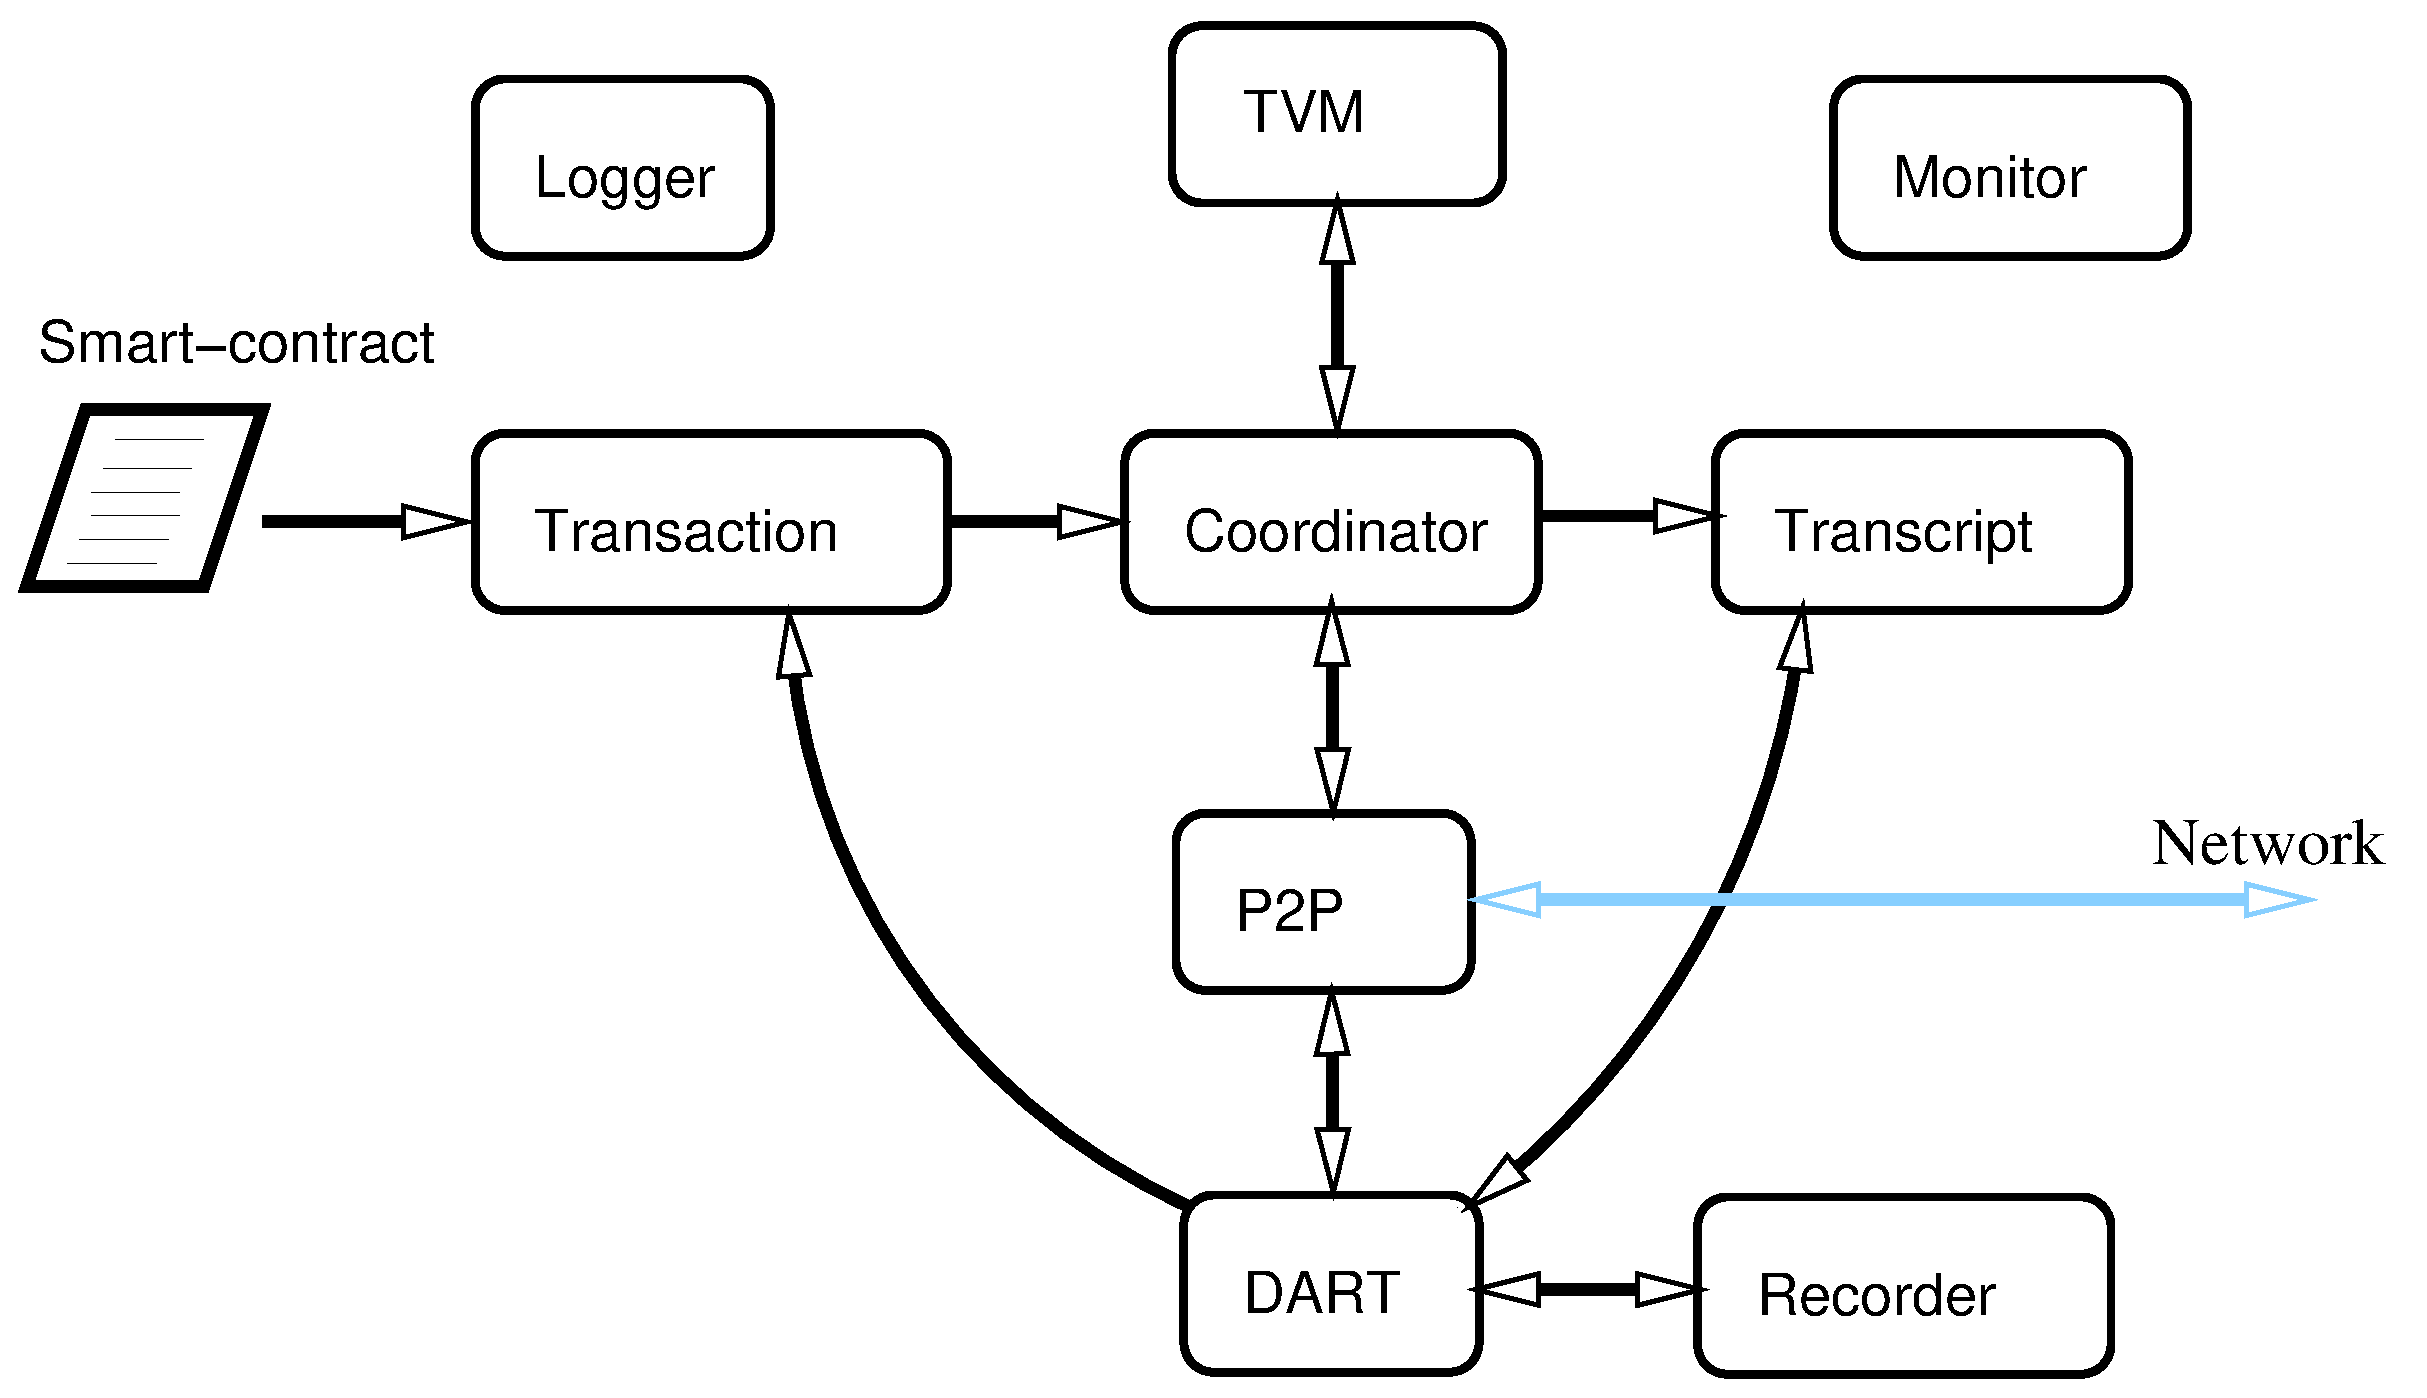
\includegraphics[width=0.8\textwidth]{fig/node_service.eps}
	% dart_bw.eps: 17766x12625 px, 300dpi, 150.42x106.89 cm, bb=0 0 4264 3030
	\caption{The Tagion Node Architure}
	\label{fig:node_service}
\end{figure}


Each of the services is running as independent tasks and communication between each-other via commutation channels. The different services modules perform the service as described in the list below.

\begin{itemize}
	\item[\bfit{Coordinator}] This service manages the hashgraph-consensus and controls other related service for the node. 
	The Coordinator generates and receives events and relays to the network. This service also generates the epoch and sends the information to the ScriptingEngine services.
	\item[\bfit{Transaction}] This service receives the incoming transaction script, validates, verifies and fetches the data from the DART and sends the information to the Coordinator.
	\item[\bfit{DART}] Services to the Distributed-database
	\item[\bfit{P2P}] This service handles the peer-to-peer communication protocol used to communicate between the nodes
	\item[\bfit{TVM}] Handles the executions of the smart contracts
	\item[\bfit{Transcript}] Services the Epoch and orders the script execution
	\item[\bfit{Recorder}] This services recorder this history of the DART.
	\item[\bfit{Logger}] The service handles information logging for the different services
	\item[\bfit{Monitor}] The Monitor service is used to graphical monitor the activities locally via a web interface.
\end{itemize}


Estimated bandwidth requirement and the average propagation for a transaction the formulas in \cref{sec:gossip_model}.
 
From simple experimental model result.\\

Example for a network with nodes $N=11$ an event size of $E_{size}=500bytes$ and network delay of $t_{net}=300ms$ the estimated epoch propagation delay
and the bandwidth of:
\begin{align*}
n_{round} &= 2.2 \cdot ln(11) &\approx  5.27\\
t_{epoch} &= 3.5 \cdot n_{round} \cdot 300ms & \approx 5.5s \\
B &= 500bytes \cdot 11^2 &= 60500bytes \\
BW &= 8 \cdot B / (n_{round}\cdot 300ms) &\approx 28kbit/s \\
\end{align*}
And with $N=31$:
\begin{align*}
n_{round} &= 2.2 \cdot ln(31) & \approx  8.6\\
t_{epoch} &= 3.5 \cdot n_{round} \cdot 300ms & \approx 8s \\
B &= 500bytes \cdot 101^2 & \approx 481kbytes \\
BW &= 8 \cdot B / (n_{round}\cdot 300ms) &\approx 152kbit/s \\
\end{align*}
And with $N=101$:
\begin{align*}
n_{round} &= 2.2 \cdot ln(101) & \approx  10.15\\
t_{epoch} &= 3.5 \cdot n_{round} \cdot 300ms & \approx 10.6s \\
B &= 500bytes \cdot 101^2 & \approx 5.1Mbytes \\
BW &= 8 \cdot B / (n_{round}\cdot 300ms) &\approx 1.2Mbit/s \\
\end{align*}
And with $N=1001$:
\begin{align*}
n_{round} &= 2.2 \cdot ln(11) & \approx  15\\
t_{epoch} &= 3.5 \cdot n_{round} \cdot 300ms & \approx 16s \\
B &= 500bytes \cdot 1001^2 & 501Mbytes \\
BW &= 8 \cdot B / (n_{round}\cdot 300ms) &\approx 80Mbit/s \\
\end{align*}

In this example the epoch delay increases round 5s when $N$ is increased by a decade and the bandwidth requirement is increased around 50 times or more.

